\documentclass[12pt]{book}

% Paquetes comunes
% common/preamble.tex — paquetes y configuración compartida
\usepackage[utf8]{inputenc}
\usepackage[T1]{fontenc}
\usepackage{lmodern}
\usepackage{geometry}
\usepackage{graphicx}
\usepackage{xcolor}
\usepackage{hyperref}
\usepackage{parskip}
\usepackage{amsmath, amssymb}

\geometry{margin=2.5cm}
\hypersetup{
    colorlinks=true,
    linkcolor=blue,
    urlcolor=blue,
    citecolor=blue
}


% Rutas de figuras de este módulo
\graphicspath{{figures/}}

\title{Libro de Ejemplo — Módulo 1}
\author{Autor del Diplomado}
\date{\today}

\begin{document}
\frontmatter
\maketitle

\tableofcontents

\mainmatter

\chapter{Introducción}
Este es un \textbf{monorepo} de ejemplo con un libro y un formato tipo Cornell.
Compila con \texttt{latexmk} y genera artefactos en \texttt{latex.out/}.

\section{Figura de ejemplo}
La Figura~\ref{fig:plot} se incluye desde \texttt{figures/ejemplo\_plot.png}.

\begin{figure}[h]
    \centering
    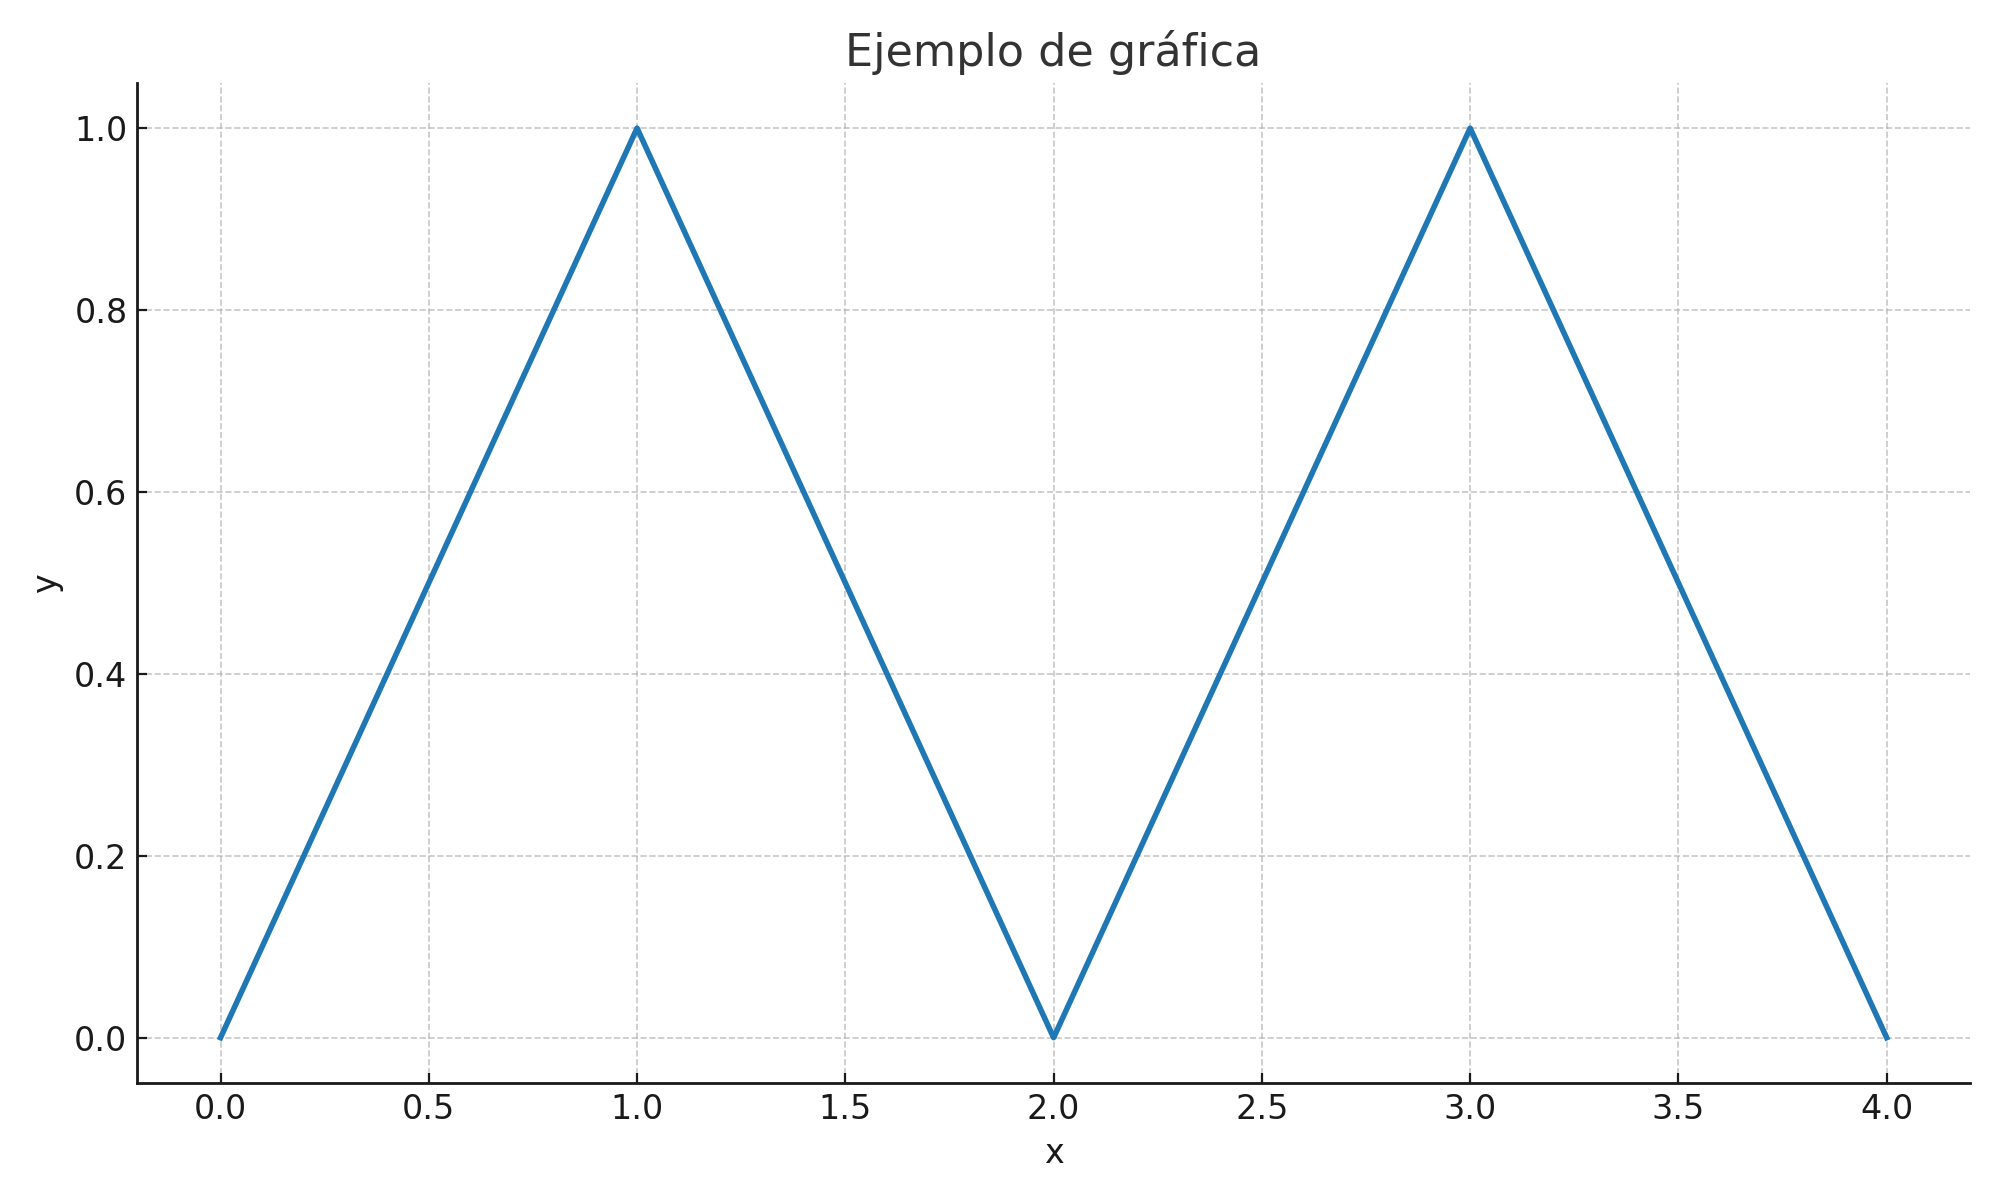
\includegraphics[width=0.7\linewidth]{ejemplo_plot.png}
    \caption{Gráfica de ejemplo generada automáticamente.}
    \label{fig:plot}
\end{figure}

\chapter{Contenido separado}
\begin{titlepage}
\newgeometry{left=7.5cm} %defines the geometry for the titlepage
\pagecolor{titlepagecolor}
\noindent
{\Huge{\textcolor{white}{Diplomado Ciencia de Datos con Python}}} \\[-1em]

\begin{figure}[h]
    \centering
    
\includegraphics[width=0.7\linewidth]{logo.png}
\end{figure}

\color{white}
\makebox[0pt][l]{\rule{1.3\textwidth}{1pt}}
\par
\noindent
%\textbf{\textsf{Diplomado Ciencia de Datos con Python}} %\textcolor{namecolor}{\textsf{Ingenier\'ia}}
\vfill
\noindent
{\huge \textsf{Módulo 1, Versión 0.0.1}}
\vskip\baselineskip
\noindent
\textsf{\today}
\end{titlepage}
\restoregeometry % restores the geometry
\nopagecolor% Use this to restore the color pages to white
%
\section*{Dedicatoria}
A quienes disfrutan de \LaTeX{}, el versionado limpio y los documentos reproducibles.

\section*{Autoría}
Autor: Nombre del autor.\\
Contacto: autor@correo.com


\backmatter
\end{document}
